\documentclass[12pt,a4paper,titlepage]{scrartcl}

\usepackage{comment}
\usepackage[main=ngerman,english]{babel}
\usepackage[utf8]{inputenc}
\usepackage[T1]{fontenc}
\usepackage{lmodern}
\usepackage{geometry}
\geometry{left=2.5cm,right=2.5cm,top=2.5cm,bottom=3cm,head=29pt,foot=25pt}
\setlength{\footheight}{25pt}
\usepackage{microtype}
\usepackage{amsmath,amssymb,mathtools}
\numberwithin{equation}{section}
\numberwithin{table}{section}
\numberwithin{figure}{section}
\usepackage{siunitx}
\sisetup{locale=US, separate-uncertainty=true, per-mode=fraction}
\usepackage{booktabs}
\usepackage{multirow}
\usepackage{graphicx}
\usepackage{float}
\usepackage{caption}
\usepackage{subcaption}
\usepackage[automark]{scrlayer-scrpage}
\usepackage[most]{tcolorbox}
\usepackage{hyperref}
\usepackage{pdfpages}
\usepackage{csvsimple-l3}
\usepackage{longtable}
\usepackage{graphicx}

%\input{../../jupyterpackages.tex}

% jupyter nbconvert --to latex 'Path'
% enferne usepackages und begin{document} und end{document}
% \input in main.tex mit \input{Path}


\newcommand{\pdfabbildung}[2]{%
    \refstepcounter{figure}%
    \addcontentsline{lof}{figure}{\protect\numberline{\thefigure}#1}%
    \label{#2}%
}

\newcommand{\pdftabelle}[2]{%
    \refstepcounter{table}%
    \addcontentsline{lot}{table}{\protect\numberline{\thetable}#1}%
    \label{#2}%
}


\hypersetup{colorlinks=true, linkcolor=blue!60!black, urlcolor=blue!60!black, citecolor=blue!60!black}

\clearpairofpagestyles

\chead{%
    \versuch\hfill\autor\\
    \rule{\textwidth}{0.2pt}%
}
\cfoot{%
    \rule{\textwidth}{0.2pt}\\[-0.5ex]
    \pagemark\ 
}
\addtokomafont{pagefoot}{\small}
\setlength{\parindent}{0pt}

\newtcolorbox{resultbox}[1][]{ 
    enhanced,
    colback=black!4!white,
    colframe=black!65!black,
    boxrule=0.8pt,
    arc=0.0mm,
    title=#1,
    fonttitle=\bfseries,
    %drop shadow
}


\newcommand{\versuch}{Versuch 14}
\newcommand{\titel}{Mathematisches Pendel}
\newcommand{\praktikum}{Physikalisches Anfängerpraktikum 1}
\newcommand{\autor}{Jonathan Gießen}
\newcommand{\gruppe}{Gruppe 8}
\newcommand{\datum}{25. September 2026}
\newcommand{\betreuer}{David Chaves}

\begin{document}

\pagestyle{scrheadings}

\begin{titlepage}



    \centering
    \vspace*{4cm}
    {\large Universität Heidelberg\par}
    {\small Fakultät für Physik und Astronomie\par}
    {\Large \praktikum\par}
    \vspace{0.8cm}
    {\LARGE \bfseries \versuch\ -- \titel\par}
    \vspace{1.5cm}

    \begin{tabular}{ll}
        \textbf{Autor:} & \autor\\
        \textbf{Gruppe:} & \gruppe\\
        \textbf{Betreuer:} & \betreuer\\
        \textbf{Versuchsdatum:} & \datum\\
    \end{tabular}

    \vfill
    \hrulefill\
\end{titlepage}

\tableofcontents

\bigskip
\begin{tcolorbox}[colback=gray!5,colframe=gray!60,boxrule=0.8pt,arc=0.01mm,title=KI-Hinweis]
    Für die sprachliche Formulierung dieses Protokolls wurde in der Einleitung \ref{sec:Einleitung} und \ref{sec:Grundlagen} KI-gestützte Textgenerierung verwendet. 
\end{tcolorbox}

\clearpage


\section{Einleitung}\label{sec:Einleitung}
Das physikalische Praktikum zum mathematischen Pendel zielt auf die präzise Bestimmung der Schwerebeschleunigung $g$ ab. Da das idealisierte Modell eines punktförmigen Pendels ohne Reibung in der Realität nicht existiert, reicht eine einfache Betrachtung für hochgenaue Messungen nicht aus. Ziel dieses Versuches ist es, durch präzise Längen- und Zeitmessungen sowie die systematische Berücksichtigung sämtlicher relevanter Störeffekte (wie Ausdehnung des Pendelkörpers, Auftrieb in der Luft, Masse des Fadens, endliche Auslenkung und Luftreibung) einen experimentellen Wert für $g$ zu ermitteln, der dem Heidelberger Standard-Wert von $g = (9,80984 \pm 2 \cdot 10^{-5}) \, \text{m/s}^2$ möglichst nahekommt. 


\section{Grundlagen und Theorie}\label{sec:Grundlagen}


\subsection{Das ideale mathematische Pendel}
In der einfachsten Näherung wird das Pendel als punktförmige Masse an einem masselosen Faden betrachtet, die reibungsfrei und mit unendlich kleiner Amplitude schwingt. Die Schwingungsdauer $T_0$ eines solchen idealen mathematischen Pendels hängt nur von der Pendellänge $l$ und der Schwerebeschleunigung $g$ ab:
\begin{equation}
    T_0 = 2\pi \sqrt{\frac{l}{g}}
    \label{eq:T0}
\end{equation}
Durch Umstellen lässt sich die Erdbeschleunigung $g$ direkt berechnen:
\begin{equation}
    g = 4\pi^2 \frac{l}{T_0^2}
    \label{eq:g_ideal}
\end{equation}

\subsection{Das physikalische Pendel und das Trägheitsmoment}
Eine exakte Theorie erfordert die Behandlung des Schwerependels als physikalisches Drehpendel, dessen Schwingungsmittelpunkt der Aufhängepunkt $P$ ist. Die Schwingungsdauer $T_D$ einer solchen Drehschwingung ist gegeben durch:
\begin{equation}
    T_D = 2\pi \sqrt{\frac{J}{D}}
    \label{eq:TD}
\end{equation}
Hierbei ist $J$ das Gesamtträgheitsmoment bezüglich der Drehachse und $D$ die Winkelrichtgröße. Das Trägheitsmoment $J_{\text{ges}}$ setzt sich nach dem Steiner'schen Satz aus den Beiträgen der Kugel (Masse $m_K$, Radius $r$) und des Fadens (Masse $m_F$, Länge $l'$) zusammen. Mit der Pendellänge $l$ (Abstand Aufhängung bis Kugelmitte) ergibt sich:
\begin{equation}
    J_{\text{ges}} = J_{\text{Kugel}} + J_{\text{Faden}} = m_K l^2 + \frac{2}{5}m_K r^2 + \frac{1}{3}m_F l'^2
    \label{eq:J_ges}
\end{equation}

\subsection{Rückstellendes Drehmoment und Winkelrichtgröße}
Wird das Pendel um den Winkel $\varphi$ aus der Ruhelage ausgelenkt, erzeugen die Gewichtskräfte ein rücktreibendes Drehmoment $M$. Bei hochpräzisen Messungen muss hierbei berücksichtigt werden, dass das Gewicht der Kugel durch den statischen Auftrieb der Luft (Dichte $\rho_L$, Kugelvolumen $V_K$) verringert wird. Der Auftrieb des dünnen Fadens wird als vernachlässigbar angenommen. Das Drehmoment lautet:
\begin{equation}
    M = - \left[ (m_K - \rho_L V_K)g \sin \varphi \cdot l + \frac{1}{2} m_F g \sin \varphi \cdot l' \right]
    \label{eq:Drehmoment}
\end{equation}
Für kleine Winkel gilt die Kleinwinkelnäherung $\sin \varphi \approx \varphi$. Setzt man zudem $m_K = \rho_K V_K$, vereinfacht sich der Ausdruck zu:
\begin{equation}
    M = - \left[ m_K \left(1 - \frac{\rho_L}{\rho_K}\right) + \frac{1}{2}m_F \right] g l \varphi
\end{equation}
Durch Vergleich mit der Definition der Winkelrichtgröße $M = -D\varphi$ erhält man:
\begin{equation}
    D = m_K g l \left[ 1 - \left( \frac{\rho_L}{\rho_K} - \frac{1}{2}\frac{m_F}{m_K} \right) \right]
    \label{eq:D_Richtgroesse}
\end{equation}

\subsection{Korrekturterme der Schwingungsdauer}
Setzt man die Gleichungen \eqref{eq:J_ges} und \eqref{eq:D_Richtgroesse} in \eqref{eq:TD} ein und wertet den Bruch $J/D$ mit Hilfe der Näherungsformel $\frac{1}{1-\epsilon} \approx 1+\epsilon$ (für kleine $\epsilon \ll 1$) aus, so ergibt sich eine erste korrigierte Schwingungsdauer in 1. Ordnung:
\begin{equation}
    T_1^2 = 4\pi^2 \frac{l}{g} \left( 1 + \frac{2}{5}\frac{r^2}{l^2} + \frac{\rho_L}{\rho_K} - \frac{1}{6}\frac{m_F}{m_K} \right)
    \label{eq:T1}
\end{equation}
Hierbei wurden Terme höherer Ordnung (wie das Produkt aus Auftriebs- und Fadengeometrieeffekten) als hinreichend klein vernachlässigt.

Da die Annahme verschwindend kleiner Amplituden experimentell nicht realisierbar ist, muss der endliche Startwinkel $\varphi_0$ berücksichtigt werden (herleitbar über den Energiesatz und die Lösung des elliptischen Integrals). Dies liefert die zweite Näherung:
\begin{equation}
    T_2^2 = T_1^2 \left( 1 + \frac{\varphi_0^2}{8} \right)
    \label{eq:T2}
\end{equation}

Zusätzlich erfährt das Pendel durch Luftreibung eine Dämpfung. Die Amplitude fällt exponentiell nach dem Gesetz $a(t) = a_0 e^{-\delta t}$ ab. Die Dämpfungskonstante $\delta$ verlängert die Periodendauer gemäß:
\begin{equation}
    T_3^2 = T_2^2 \left[ 1 + \left(\frac{\delta^2}{\omega_2^2}\right) \right]
    \label{eq:T3}
\end{equation}

\subsection{Gesamtgleichung der Periodendauer}
Setzt man alle Korrekturterme zusammen, so ergibt sich für die gemessene, reale Schwingungsdauer $T_g$:
\begin{equation}
    T_g^2 = 4\pi^2 \frac{l}{g} \left( 1 + \frac{2}{5}\frac{r^2}{l^2} + \frac{\rho_L}{\rho_K} - \frac{1}{6}\frac{m_F}{m_K} + \frac{\delta^2}{\omega_0^2} + \frac{\varphi_0^2}{8} \right)
    \label{eq:T_gesamt}
\end{equation}
Diese Gleichung ermöglicht es, aus der real gemessenen Zeit und den geometrischen Abmessungen den hochpräzisen Wert für $g$ zu extrahieren.

\subsection{Fehlerbetrachtung und optimale Messzeit}
Die Genauigkeit der berechneten Schwerebeschleunigung wird maßgeblich durch die Fehler der Längenmessung ($\Delta l$) und der Zeitmessung ($\Delta t$) dominiert. Misst man $n$ Schwingungen, beträgt der relative Fehler der Einzelperiode $\frac{\Delta T_0}{T_0} = \frac{\Delta t}{n T_0}$.
Für den relativen Gesamtfehler von $g$ folgt nach dem Fehlerfortpflanzungsgesetz:
\begin{equation}
    \frac{\Delta g}{g} = \sqrt{ \left(\frac{\Delta l}{l}\right)^2 + \left(\frac{2\Delta t}{n T_0}\right)^2 }
    \label{eq:Fehler_g}
\end{equation}
Es ist physikalisch nicht sinnvoll, die Zeitmessung durch eine extrem hohe Schwingungszahl $n$ viel präziser als die Längenmessung zu machen. Eine optimierte Abstimmung der Fehlerbeiträge ergibt sich durch die Forderung, dass der Fehler der Zeitmessung etwa 30\% des Längenfehlers ausmachen soll:
\begin{equation}
    \frac{2\Delta t}{n T_0} \approx 0,3 \frac{\Delta l}{l}
    \label{eq:n_opt}
\end{equation}
Aus dieser Bedingung lässt sich die ideale Anzahl $n$ der zu messenden Schwingungsdurchgänge vorab abschätzen.

\subsection{Fehlerfortpflanzung nach Gauß}
Für die Fehlerrechnung wird die Gaußsche Fehlerfortpflanzung verwendet. Für eine Funktion $f(x_1, x_2, \dots, x_n)$ mit den unabhängigen Variablen $x_i$ und den zugehörigen Standardabweichungen $\sigma_{x_i}$ gilt:
\begin{equation}
    \sigma_f = \sqrt{\sum_{i=1}^{n} \left(\frac{\partial f}{\partial x_i} \sigma_{x_i}\right)^2}
\end{equation}

Fehler gleicher Einheit werden quadratisch addiert:

\begin{equation}
    \sigma_f = \sqrt{\sigma_{x_1}^2 + \sigma_{x_2}^2}
\end{equation}

Fehler unterschiedlicher Einheitwerden über die partielle Ableitung der Funktion gewichtet.\footnote{Die bechnungen werden mit der Python-Bibliothek \texttt{uncertainties} durchgeführt, welche die Gaußsche Fehlerfortpflanzung automatisch implementiert. Code ist im Anhang.}


\subsection{Literaturwerte}

Die Erdbeschleunigung $g$ variiert je nach geographischer Lage. Für Heidelberg beträgt der Standardwert:
\begin{equation}
    g_{\text{Heidelberg}} = \qty{9.80984(2)}{\meter\per\second\squared}
\end{equation}


    
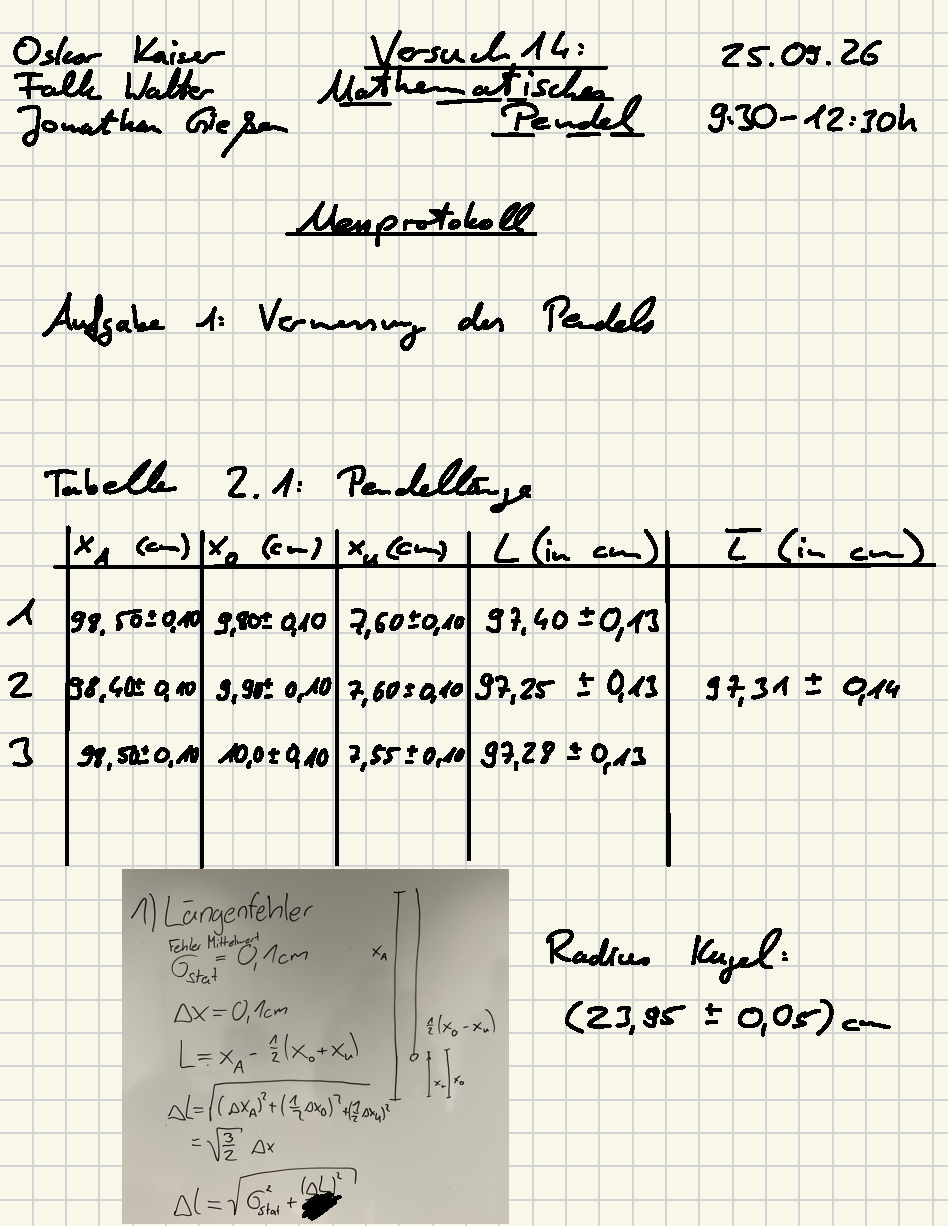
\includepdf[
    pages=-,
    width=\textwidth,
    height=0.95\textheight,
    keepaspectratio,
    pagecommand={\thispagestyle{scrheadings}},
    pagecommand*={\thispagestyle{scrheadings}\section{Messprotokoll}\subsection{Versuchsaufbau und Aufgaben}}
]{../Messprotokoll 14.pdf}

\subsection{Durchführung}
Messung der Fadenlänge des Pendels und dem Daraus resultierendem Fehler der Längenmessung. Anschließend Messung der Schwingungsdauer für eine bestimmte Anzahl an Schwingungen, um den Fehler der Zeitmessung zu bestimmen. 
Daraus berechnet sich nach Gleichung \eqref{eq:n_opt} die optimale Anzahl an Schwingungen $n$, die für die Messung der Schwingungsdauer durchgeführt werden sollte.
Im folgenden wurde die Messung der Schwingungsdauern $n$ 2 mal durchgeführt, dabei wurde die Amplitude des Pendels in Zeitabständen notiert, um die Dämpfungskonstante $\delta$ zu bestimmen. Um das Physikalische Pendel besser zu bestimmen, wurde der Durchmesser der Kugel gemessen, um später die Masse aus der Dichte von Eisen zu bestimmen


\section{Auswertung}

\subsection{Aufgabe 1: Mathematisches Pendel}
Mithilfe von Gleichung \ref{eq:g_ideal} kann die Schwerebeschleunigung $g$ aus den gemessenen Werten berechnet werden.

Die gemessenen Werte betragen: 
\begin{table}[H]
    \centering
    \caption{Messwerte des Mathematischen Pendels.}
    \begin{tabular}{lc}
        \toprule
        \textbf{Größe} & \textbf{Wert} \\
        \midrule
        Fadenlänge & $L = \qty{97.31(14)e-2}{\meter}$ \\
        Anzahl der Schwingungen & $n = 514$ \\
        Schwingungsdauer & $T = \qty{972.55(22)}{\second}$ \\
        Periodendauer & $T_0 = \qty{1.89(22)}{\second}$ \\
        \bottomrule
    \end{tabular}
\end{table}

Aus den gemessenen Werten ergibt sich für die Schwerebeschleunigung:
\begin{equation}
    g_\text{mat} = \qty{10.7(2.4)}{\meter\per\second\squared}
\end{equation}

Die Abweichung vom Literaturwert beträgt:
\begin{equation}
    \sigma g_\text{mat} = \frac{\lvert g_\text{mat} - g_\text{Heidelberg}\rvert}{\sqrt{\sigma g_\text{mat}^2 + \sigma g_\text{Heidelberg}^2}} \Rightarrow 0.38\sigma
\end{equation}

\begin{resultbox}[Ergebnis Aufgabe 1]
    \begin{equation}
        g_\text{mat} = \qty{10.7(2.4)}{\meter\per\second\squared} \Rightarrow 0.38\sigma
    \end{equation}
\end{resultbox}

\bigskip
\subsection{Aufgabe 2: Physikalisches Pendel}

\subsubsection{Bestimmung der Dämpfungskonstante}

Durch Auftragen der Messwerte der Amplitude in einen Halblogarithmischen Plot gegen die Zeit, kann durch eine Exponentialfunktion eine Ausgleichsgerade ermittelt werden, die die Dämpfungskonstante $\delta$ beschreibt. Die Messwerte und der Fit sind in Abbildung \ref{fig:amplitude_fit} dargestellt.

\begin{figure}[H]
    \centering
    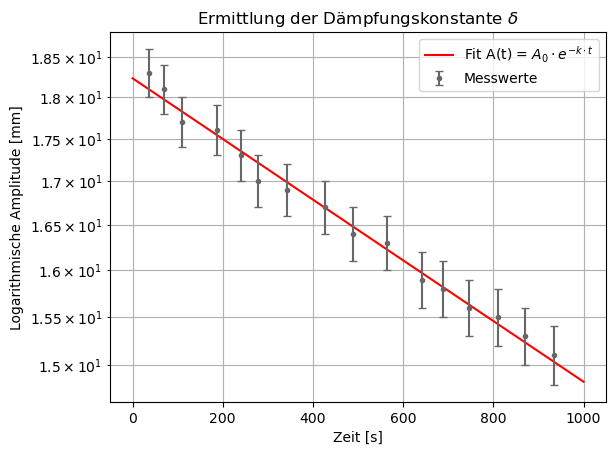
\includegraphics[width=0.8\textwidth]{img/Damping.png}
    \caption{Halblogarithmischer Plot der Amplitude gegen die Zeit mit Fit zur Bestimmung der Dämpfungskonstante $\delta$.}
    \label{fig:amplitude_fit}
\end{figure}

Die Ausgleichgerade schreibt sich nach der Funktion:
\begin{align}
    A(t) &= A_0 e^{-\delta t}\\
    A(t) &= \qty{18.23(6)}{\milli\meter} \cdot exp\left(-\qty{2.06(6)e-4}{\per\second}\,t\right)
\end{align}

Die Dämpfungskonstante beträgt somit:
\begin{equation}
    \delta = \qty{2.06(6)e-4}{\per\second}
\end{equation}

Der Fehler der Dämpfungskonstante ergibt sich aus der Covarianzmatrix des Fits.

\subsubsection{Längenverhältnis von Faden und Kugelradius}

Dieser Korrekturterm lässt sich durch die Formel:

\begin{align}
    k_1 &= \frac{2}{5}\frac{r^2}{l^2}\\
    \Delta k_1 &= \sqrt{\left(\frac{4}{5}\frac{r}{l^2}\Delta r\right)^2 + \left(\frac{4}{5}\frac{r^2}{l^3}\Delta l\right)^2}
\end{align}

bestimmen. 

Mit der Fadenlänge $l = \qty{97.31(14)e-2}{\meter}$ und dem Kugelradius $r = \qty{23.95(5)e-3}{\meter}$ ergibt sich:
\begin{equation}
    k_1 = \num{2.423(13)e-4}
\end{equation}

\subsection{Korrektur für den Auftrieb}
Aufgrund des Auftriebs der Luft, der die Gewichtskraft der Kugel verringert, muss eine Korrektur vorgenommen werden. Der Korrekturterm lässt sich durch die Formel:

\begin{align}
    k_2 &= \frac{\rho_L}{\rho_K}\\
    \Delta k_2 &= \sqrt{\left(\frac{1}{\rho_K}\Delta \rho_L\right)^2 + \left(\frac{\rho_L}{\rho_K^2}\Delta \rho_K\right)^2}
\end{align}

bestimmen.

Die Luftdichte lässt sich googlen oder wenn man Hobbylos ist berechnen\footnote{Die Werte kommen von den Freunden des Millikanversuchs}:
\begin{equation}
    \rho_L = \frac{p}{R_s*T} = \frac{\qty{100990(20)}{Pa}}{\qty{287.05}{\joule\per\kilo\gram\kelvin} * \qty{294.15(1.00)}{\kelvin} } = \qty{1.196(4)}{\kilo\gram\per\meter\cubed}
\end{equation}

mit 

\begin{equation}
    \delta \rho_L = \sqrt{\left(\frac{1}{R_s*T}\Delta p\right)^2 + \left(\frac{p}{R_s*T^2}\Delta T\right)^2}
\end{equation}

Es ergibt sich somit für den Korrekturterm mit $\rho_L = \qty{1.196(4)}{\kilo\gram\per\meter\cubed}$ und $\rho_K = \qty{7.86e3}{\kilo\gram\per\meter\cubed}$:
\begin{equation}
    k_2 = \frac{\rho_L}{\rho_K} = \frac{\qty{1.196(4)}{\kilo\gram\per\meter\cubed}}{\qty{7.87e3}{\kilo\gram\per\meter\cubed}} = \num{1.521(6)e-4}
\end{equation}

\subsection{Korrektur für die Fadenmasse}

Der Korrekturterm für die Fadenmasse lässt sich durch die Formel:
\begin{align}
    k_3 &= \frac{1}{6}\frac{m_F}{m_K}\\
    \Delta k_3 &= \sqrt{\left(\frac{1}{6 m_K}\Delta m_F\right)^2 + \left(\frac{m_F}{6 m_K^2}\Delta m_K\right)^2}
\end{align}
bestimmen.


\clearpage

\listoffigures


\listoftables

\begin{thebibliography}{5}
    \bibitem{PAPskript} Dr. J.Wagner, \emph{Physikalisches Anfängerpraktikum}, Stand 11/2024
    \bibitem{ilberg1988physikalisches} W. Ilberg, M. Krötzsch, \emph{Physikalisches Praktikum für Anfänger}, BSB B. G. Teubner Verlagsgesellschaft, Leipzig (1985).
\end{thebibliography}




\begin{comment}

\begin{table}[H]
    \centering
    \caption{Mess- und Geräteparameter für die exemplarische Berechnung (Messung 28).}
    \label{tab:parameter_messung_28}
    \begin{tabular}{ll}
        \toprule
        \textbf{Größe} & \textbf{Wert} \\
        \midrule
        Fallstrecke & $s_1 = 10\,\text{Skt} = 5.00 \cdot 10^{-4}\,\text{m}$ \\
        Fallzeit & $t_1 = 11.85\,\text{s}$ \\
        Steigstrecke & $s_2 = 10\,\text{Skt} = 5.00 \cdot 10^{-4}\,\text{m}$ \\
        Steigzeit & $t_2 = 18.19\,\text{s}$ \\
        Skalenteilung & $1\,\text{Skt} = 5.00 \cdot 10^{-5}\,\text{m}$ \\
        Kondensatorspannung & $U = 500\,\text{V}$ \\
        Plattenabstand & $d = 6.00 \cdot 10^{-3}\,\text{m}$ \\
        Luftdruck & $p = 100285\,\text{Pa}$ \\
        Erdbeschleunigung & $g = 9.81\,\frac{\text{m}}{\text{s}^2}$ \\
        Dichtedifferenz & $\rho = \rho_{\text{Öl}} - \rho_{\text{Luft}} = 871.21\,\frac{\text{kg}}{\text{m}^3}$ \\
        Unkorrigierte Luftviskosität & $\eta_0 = 1.81 \cdot 10^{-5}\,\text{Pa}\cdot\text{s}$ \\
        Cunningham-Konstante & $b = 7.78 \cdot 10^{-3}\,\text{Pa}\cdot\text{m}$ \\
        \bottomrule
    \end{tabular}
\end{table}
\end{comment}
\end{document}